\chapter{Конструкторская часть}
%<пишем про алгоритмы, архитектуру ПО>
\section{Диаграмма проектируемой базы данных}
На рисунке~\ref{fig:db} представлена диаграмма проектируемой базы данных.

\begin{figure}[H]
	\centering
	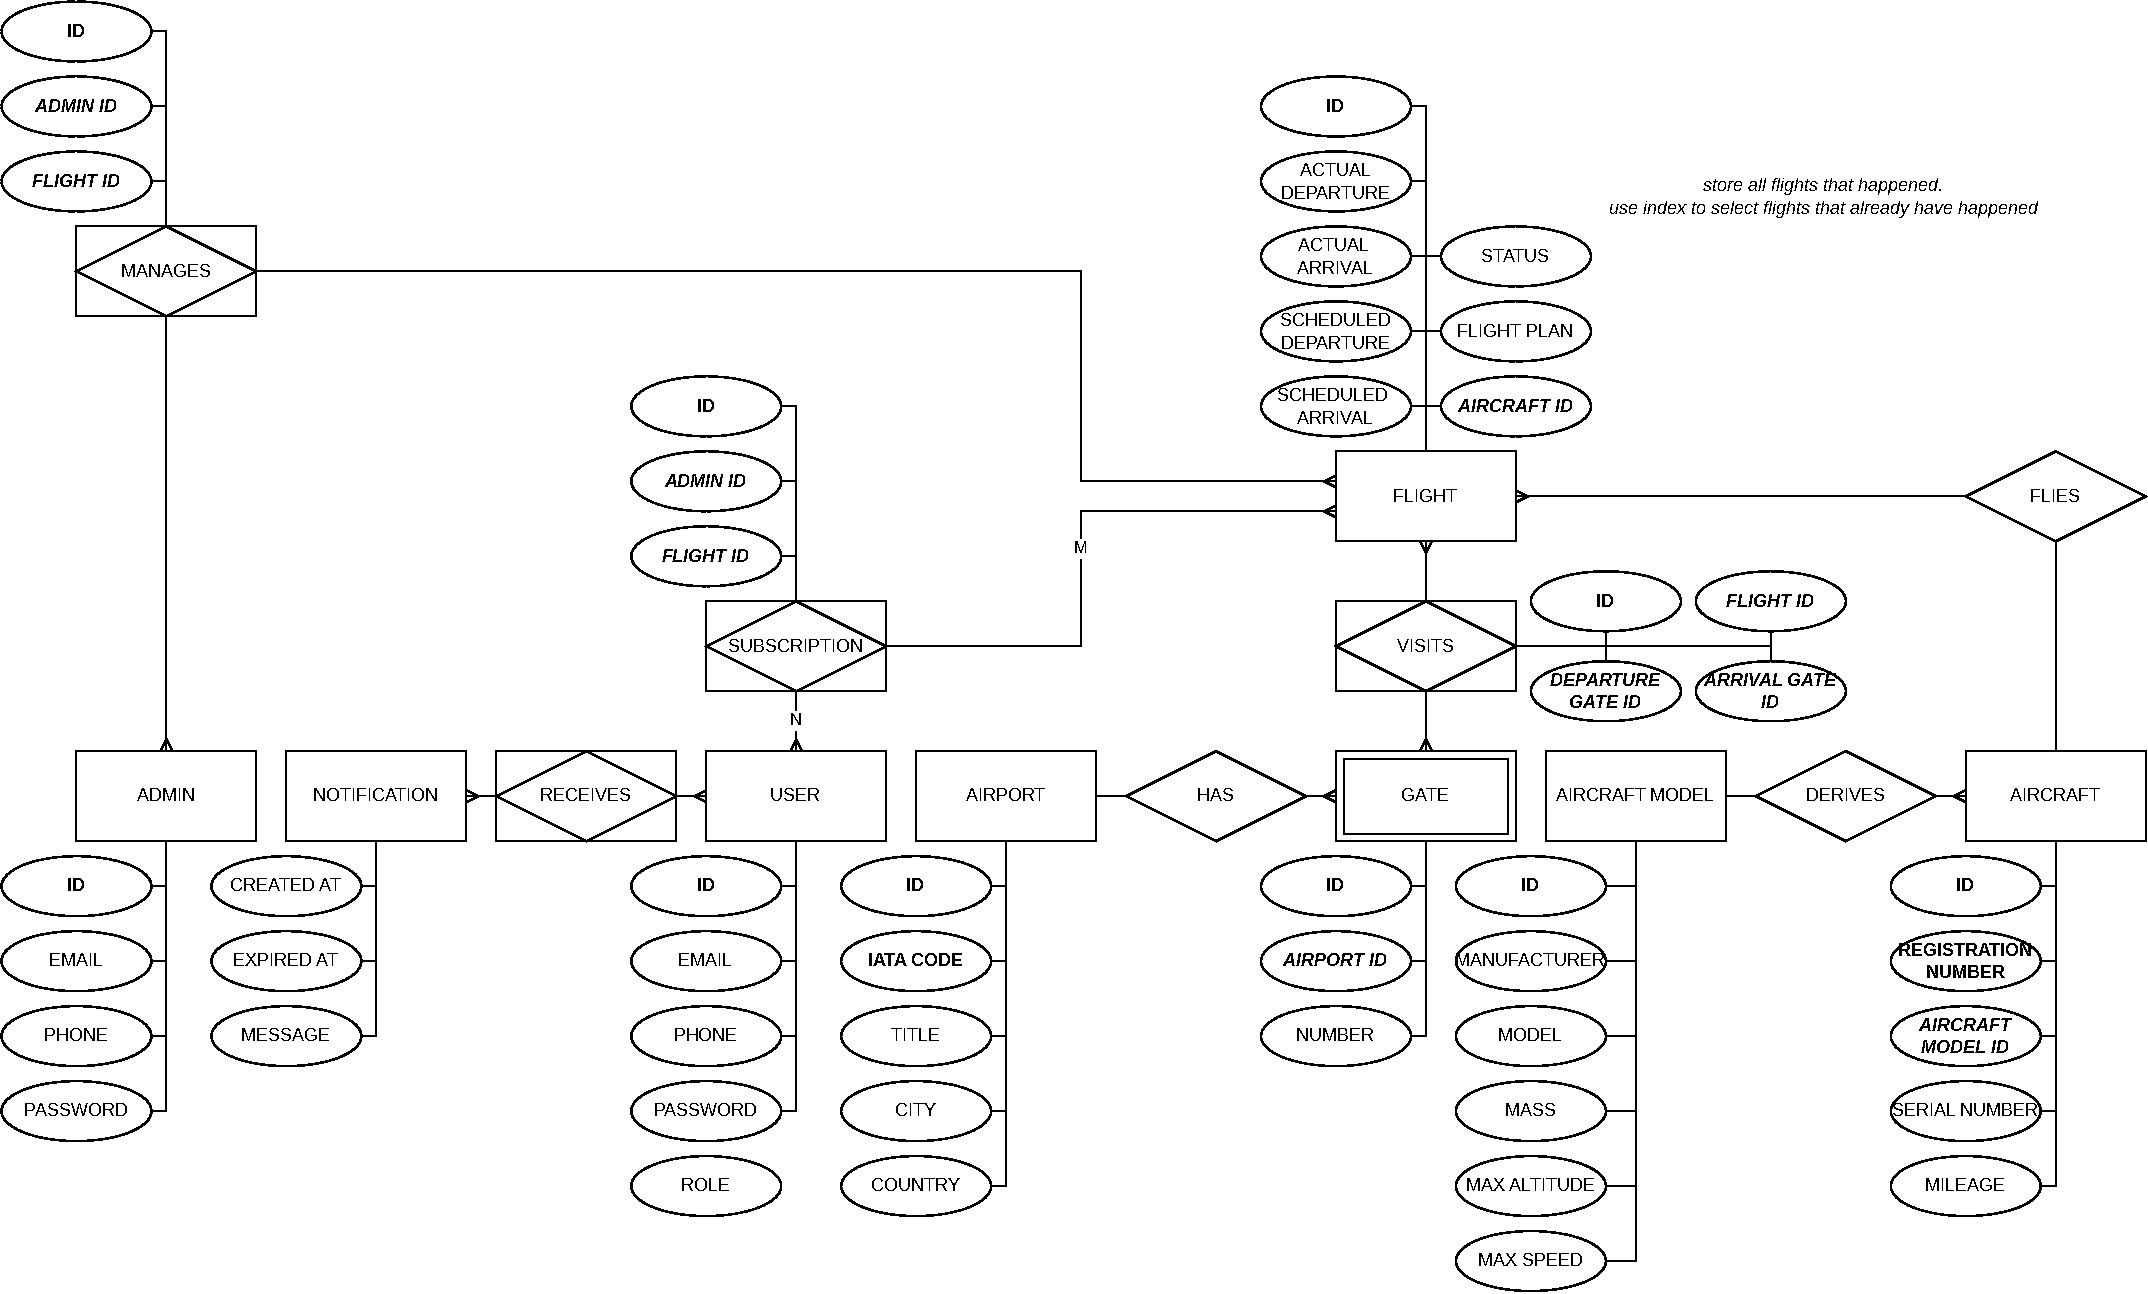
\includegraphics[height=0.7\textheight]{diags/db.pdf}
	\caption{Диаграмма базы данных}
	\label{fig:db}
\end{figure}

\section{Доказательство что спроектированная база данных находится в 3НФ}
...

\section{Описание сущностей проектируемой базы данных}
Сущностями базы данных являются: пользователь, аэропорт, выход аэропорта, модель самолёта, самолёт, рейсы. Сущность пользователь отображает представление пользователя приложения, с помощью атрибута role происходит разграничени администратора и обычного пользователя. Сущности aircraft и aircraft\_models отображают информацию по самолёте. Сущности airports и gates отображают информацию об аэропорте. Сущности flights и visits отображают информацию о рейсе.

\section{Описание проектируемых ограничений целостности базы данных}

\section{Описание всех проектируемых процедур/функций/триггеров в формате схемы}

\section{Описание проектируемой ролевой модели на уровне базы данных (у каких ролей какой доступ и к каким объектам)}

\clearpage